\documentclass{article}
\usepackage[utf8]{inputenc}
\usepackage{hyperref}
\usepackage[letterpaper, portrait, margin=1in]{geometry}
\usepackage{enumitem}
\usepackage{amsmath}
\usepackage{amsthm}
\usepackage{booktabs}
\usepackage{graphicx}
\usepackage{float}
\usepackage{hyperref}
\usepackage[flushleft]{threeparttable}
\usepackage{textcomp}
\usepackage{amssymb}
\usepackage{dsfont}
\hypersetup{
colorlinks=true,
    linkcolor=black,
    filecolor=black,      
    urlcolor=blue,
    citecolor=black,
}
\usepackage{natbib}
\usepackage{yhmath}

\usepackage{titlesec}
\bibliographystyle{chicago}
\newcommand{\bib}{references.bib}
\newcommand\iid{\stackrel{\mathclap{iid}}{\sim}}
\newcommand\asym{\stackrel{\mathclap{a}}{\sim}}
\newcommand\convprob{\xrightarrow{p}}
\newcommand\convdist{\xrightarrow{d}}
\newcommand{\N}{\mathbb{N}}
\newcommand{\Z}{\mathbb{Z}}
\newcommand{\E}{\text{E}}
\newcommand{\V}{\text{Var}}
\newcommand{\Av}{\text{Avar}}
\newcommand{\se}{\text{se}}
\newcommand{\corr}{\text{Corr}}
\newcommand{\cov}{\text{Cov}}
\newcommand{\norm}{\text{Normal}}
\newcommand{\indep}{\perp \!\!\! \perp}

\begin{document}
% The tex content below is similar to the given main.tex
 
\title{Homework 6}
\author{Environmental Economics II\\
Maghfira Ramadhani}
\date{\today}
\maketitle

\section*{Problem 1 Hourly data - Stata}
\begin{enumerate}
    \item The cohort group indicator can be generated using line 70 to 80 in the \verb!0_run_code.do!
    \item The number of negative weights is 48,547.
    \item The regression estimates is show in Table \ref{t1:TWFEDID_hr}.
    \begin{table}[H]\centering
        \caption{TWFE regression on hourly data}
        \label{t1:TWFEDID_hr}
        \begin{threeparttable}
        {
\def\sym#1{\ifmmode^{#1}\else\(^{#1}\)\fi}
\begin{tabular}{l*{1}{c}}
\hline\hline
                    &\multicolumn{1}{c}{Energy Consumption (kWh)}\\
\hline
ATT                 &     -0.0434\sym{***}\\
                    &    (0.0002)         \\
[1em]
Temperature (F)     &      0.0046\sym{***}\\
                    &    (0.0000)         \\
[1em]
Precipitation (in)  &     -0.0006         \\
                    &    (0.0020)         \\
[1em]
Relative Humidity (\%)&      0.0023\sym{***}\\
                    &    (0.0000)         \\
[1em]
Constant            &      0.5387\sym{***}\\
                    &    (0.0011)         \\
\hline
Observations        &      720000         \\
Adjusted \(R^{2}\)  &       0.663         \\
\hline\hline
\multicolumn{2}{l}{\footnotesize Standard errors in parentheses}\\
\multicolumn{2}{l}{\footnotesize \sym{*} \(p<0.10\), \sym{**} \(p<0.05\), \sym{***} \(p<0.01\)}\\
\end{tabular}
}

        \end{threeparttable}
        \end{table}
\end{enumerate}

\section*{Problem 2 Daily data - Stata}
\begin{enumerate}
    \item The regression estimates is show in Table \ref{t2:TWFEDID_day}. The coefficient does not change much from the hourly data, i.e. $ATT_{daily}=-0.9356 \approxeq 24\times ATT_{hourly}=24\times -0.0434=-1.04 $. The small difference may be due to the hourly seasonality that is not captured in the daily data. However the R-squared is higher when using the daily data indicating there is a lot of noise in the hourly electricity consumption.
    \begin{table}[H]\centering
        \caption{TWFE regression on daily data}
        \label{t2:TWFEDID_day}
        \begin{threeparttable}
        {
\def\sym#1{\ifmmode^{#1}\else\(^{#1}\)\fi}
\begin{tabular}{l*{1}{c}}
\hline\hline
                    &\multicolumn{1}{c}{Energy consumption (kWh)}\\
\hline
ATT                 &     -0.9356\sym{***}\\
                    &    (0.0056)         \\
[1em]
Temperature (F)     &      0.1109\sym{***}\\
                    &    (0.0004)         \\
[1em]
Precipitation (in)  &      0.0681         \\
                    &    (0.1882)         \\
[1em]
Relative Humidity (\%)&      0.0552\sym{***}\\
                    &    (0.0002)         \\
[1em]
Constant            &     12.8783\sym{***}\\
                    &    (0.0341)         \\
\hline
Observations        &       30000         \\
Adjusted \(R^{2}\)  &       0.971         \\
\hline\hline
\multicolumn{2}{l}{\footnotesize Standard errors in parentheses}\\
\multicolumn{2}{l}{\footnotesize \sym{*} \(p<0.10\), \sym{**} \(p<0.05\), \sym{***} \(p<0.01\)}\\
\end{tabular}
}

        \end{threeparttable}
        \end{table}
    \item The event-study regression is the following:
    \begin{align*}
        Y_{i,t}=\alpha_i+\sum_{\tau=-30}^{-2}\beta_\tau^{pre} 1(R_{i,t}=\tau)+\sum_{\tau=0}^{30}\beta_\tau^{post} 1(R_{i,t}=\tau)+\gamma X_{i,t}+\varepsilon_{i,t}
    \end{align*}
    Note that I am not adding the time fixed effect in the regression as in the instruction as it will adsorb the time variation that we want to observe in the lead and lag coefficient. The event study estimates is shown in Figure \ref{f1:event_study} which gives similar result with the canned event study in Figure \ref{f2:event_study_canned}.
    \begin{figure}[H]
        \centering
        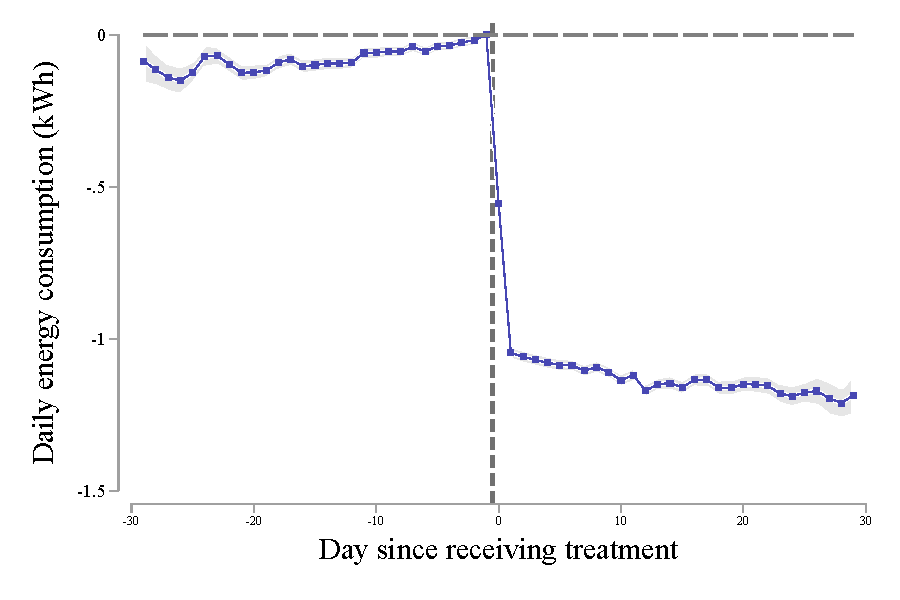
\includegraphics[width=0.7\textwidth]{./figure/event_study.pdf}
        \caption{Event study of daily data}
        \label{f1:event_study} 
        \end{figure}
    \item Figure \ref{f2:event_study_canned} show the event study estimates using the \verb!eventdd! package. 
    \begin{figure}[H]
        \centering
        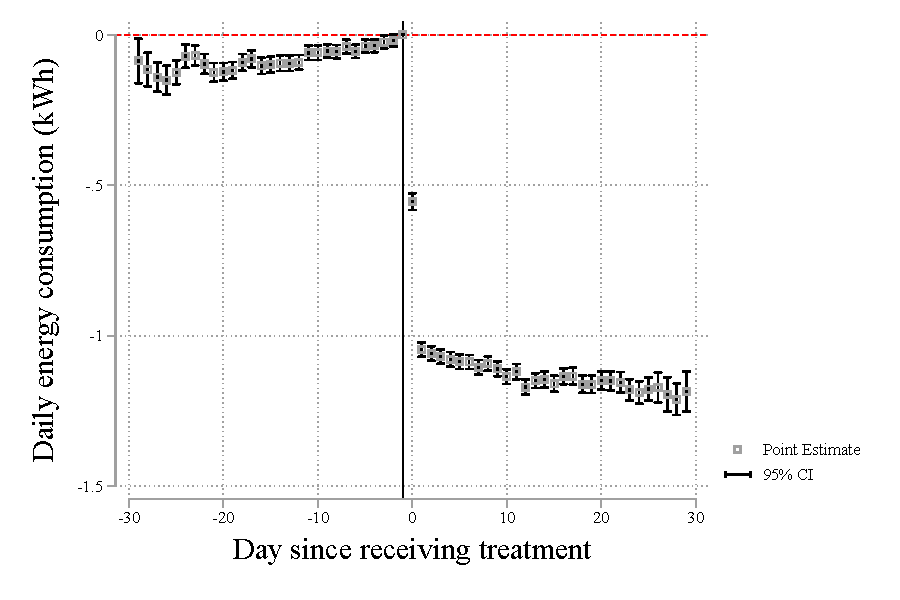
\includegraphics[width=0.7\textwidth]{./figure/event_study_canned.pdf}
        \caption{Event study of daily data using eventdd}
        \label{f2:event_study_canned} 
        \end{figure}
    \item Using the CSDID package the ATT is -1.132823. Figure \ref{f3:event_study_csdid} show the event study estimates from using the \verb!csdid! package.
    \begin{figure}[H]
        \centering
        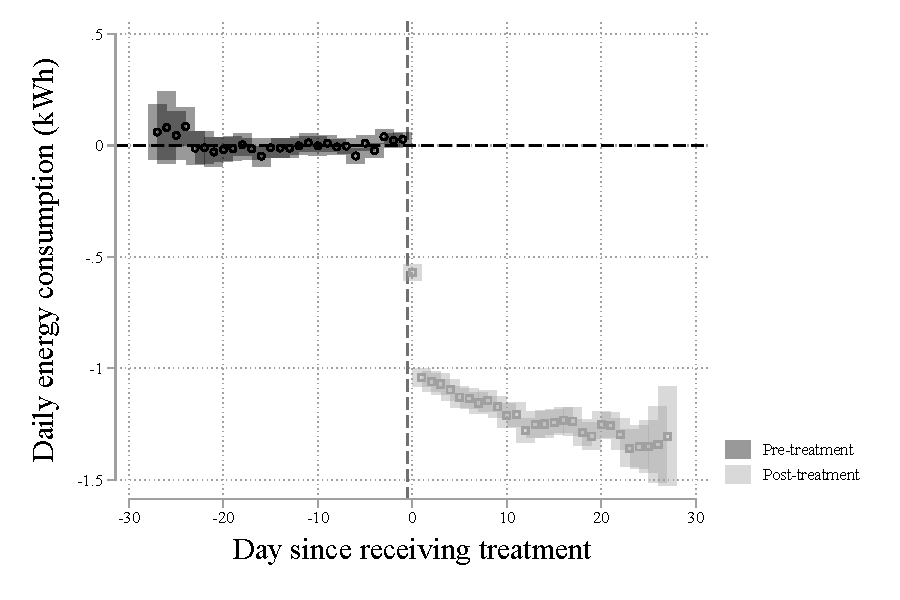
\includegraphics[width=0.7\textwidth]{./figure/event_study_csdid.pdf}
        \caption{Event study of daily data using csdid}
        \label{f3:event_study_csdid} 
        \end{figure}
\end{enumerate}

\end{document}